\hypertarget{inference}{%
\chapter{Inference}\label{inference}}

\href{https://colab.research.google.com/github/AllenDowney/ElementsOfDataScience/blob/master/11_inference.ipynb}{Click
here to run this notebook on Colab} or
\href{https://github.com/AllenDowney/ElementsOfDataScience/raw/master/11_inference.ipynb}{click
here to download it}.

This chapter introduces \textbf{statistical inference}, which is the
process of using a sample to make inferences about a population.

The \textbf{population} is the group we are interested in. Sometimes it
is a group of people, but in general it can be any kind of group.

If we can observe the entire group, we might not need statistical
inference. If not, sometimes we can observe a \textbf{sample} (or
subset) of the population and use those observations to make claims
about the population.

If you have studied statistics before, you might have encountered some
of these ideas before: hypothesis testing, p-values, estimation,
standard error, and confidence intervals.

In this chapter we'll approach these topics using computation and
simulation, as opposed to mathematical analysis. I hope this approach
makes the ideas clearer.

If you have not seen these ideas before, don't worry. That might even be
better.

We'll look at three examples:

\begin{itemize}
\item
  Testing whether a coin is ``fair''.
\item
  Testing whether first babies are more like to be born early (or late).
\item
  Estimating the average height of men in the U.S., and quantifying the
  precision of the estimate.
\end{itemize}

\hypertarget{the-euro-problem}{%
\section{The Euro problem}\label{the-euro-problem}}

In \emph{Information Theory, Inference, and Learning Algorithms}, David
MacKay writes, "A statistical statement appeared in \emph{The Guardian}
on Friday January 4, 2002:

\begin{quote}
When spun on edge 250 times, a Belgian one-euro coin came up heads 140
times and tails 110. `It looks very suspicious to me', said Barry
Blight, a statistics lecturer at the London School of Economics. `If the
coin were unbiased the chance of getting a result as extreme as that
would be less than 7\%'.*
\end{quote}

But do these data give evidence that the coin is biased rather than
fair?"

Before we answer MacKay's question, let's unpack what Dr.~Blight said:

``If the coin were unbiased the chance of getting a result as extreme as
that would be less than 7\%''.

To see where that comes from, I'll simulate the result of spinning an
``unbiased'' coin, meaning that the probability of heads is 50\%.

Here's an example with 10 spins:

\begin{lstlisting}[language=Python]
import numpy as np

spins = np.random.random(10) < 0.5
spins
\end{lstlisting}

\begin{lstlisting}[]
array([ True,  True,  True, False,  True,  True,  True,  True,  True,
       False])
\end{lstlisting}

\passthrough{\lstinline!np.random.random!} returns numbers between 0 and
1, uniformly distributed. So the probability of being less than 0.5 is
50\%.

The sum of the array is the number of \passthrough{\lstinline!True!}
elements, that is, the number of heads:

\begin{lstlisting}[language=Python]
np.sum(spins)
\end{lstlisting}

\begin{lstlisting}[]
8
\end{lstlisting}

We can wrap that in a function that simulates
\passthrough{\lstinline!n!} spins with probability
\passthrough{\lstinline!p!}.

\begin{lstlisting}[language=Python]
def spin(n, p):
    return np.sum(np.random.random(n) < p)
\end{lstlisting}

Here's an example with the actual sample size (250) and hypothetical
probability (50\%).

\begin{lstlisting}[language=Python]
heads, tails = 140, 110
sample_size = heads + tails
\end{lstlisting}

\begin{lstlisting}[language=Python]
hypo_prob = 0.5
spin(sample_size, hypo_prob)
\end{lstlisting}

\begin{lstlisting}[]
119
\end{lstlisting}

Since we are generating random numbers, we expect to see different
values if we run the experiment more than once.

Here's a loop that runs \passthrough{\lstinline!spin!} 10 times.

\begin{lstlisting}[language=Python]
n = 250
p = 0.5

for i in range(10):
    print(spin(n, p))
\end{lstlisting}

\begin{lstlisting}[]
114
121
116
131
141
139
135
129
127
133
\end{lstlisting}

As expected, the results vary from one run to the next.

Now let's run the simulated experiment 10000 times and store the results
in a NumPy array.

\begin{lstlisting}[language=Python]
outcomes = np.empty(1000)

for i in range(len(outcomes)):
    outcomes[i] = spin(n, p)
\end{lstlisting}

\passthrough{\lstinline!np.empty!} creates an empty array with the given
length. Each time through the loop, we run
\passthrough{\lstinline!spin!} and assign the result to an element of
\passthrough{\lstinline!outcomes!}.

The result is an array of 10000 integers, each representing the number
of heads in a simulated experiment.

The mean of \passthrough{\lstinline!outcomes!} is about 125:

\begin{lstlisting}[language=Python]
np.mean(outcomes)
\end{lstlisting}

\begin{lstlisting}[]
124.967
\end{lstlisting}

Which makes sense. On average, the expected number of heads is the
product of the hypothetical probability and the sample size:

\begin{lstlisting}[language=Python]
expected = hypo_prob * sample_size
expected
\end{lstlisting}

\begin{lstlisting}[]
125.0
\end{lstlisting}

Now let's see how much the values in \passthrough{\lstinline!outcomes!}
differ from the expected value:

\begin{lstlisting}[language=Python]
diffs = outcomes - expected
\end{lstlisting}

\passthrough{\lstinline!diffs!} is an array that contains the deviation
of each experiment from the expected value, 125.

Here's the mean of the absolute deviations:

\begin{lstlisting}[language=Python]
np.mean(abs(diffs))
\end{lstlisting}

\begin{lstlisting}[]
6.673
\end{lstlisting}

So a typical experiment deviates from the mean by about 6.

To see the whole distribution of deviations, we can plot a histogram.
The following function uses Matplotlib to plot a histogram and adjust
some of the settings.

\begin{lstlisting}[language=Python]
import matplotlib.pyplot as plt

def plot_hist(values):
    xs, ys, patches = plt.hist(values,
                               density=True,
                               histtype='step',
                               linewidth=2,
                               alpha=0.5)
    
    
    plt.ylabel('Density')
    plt.tight_layout()
    return patches[0]
\end{lstlisting}

Here's what the distribution of deviations looks like:

\begin{lstlisting}[language=Python]
plot_hist(diffs)

plt.title('Sampling distribution (n=250)')
plt.xlabel('Deviation from expected number of heads');
\end{lstlisting}

\begin{figure}
\centering
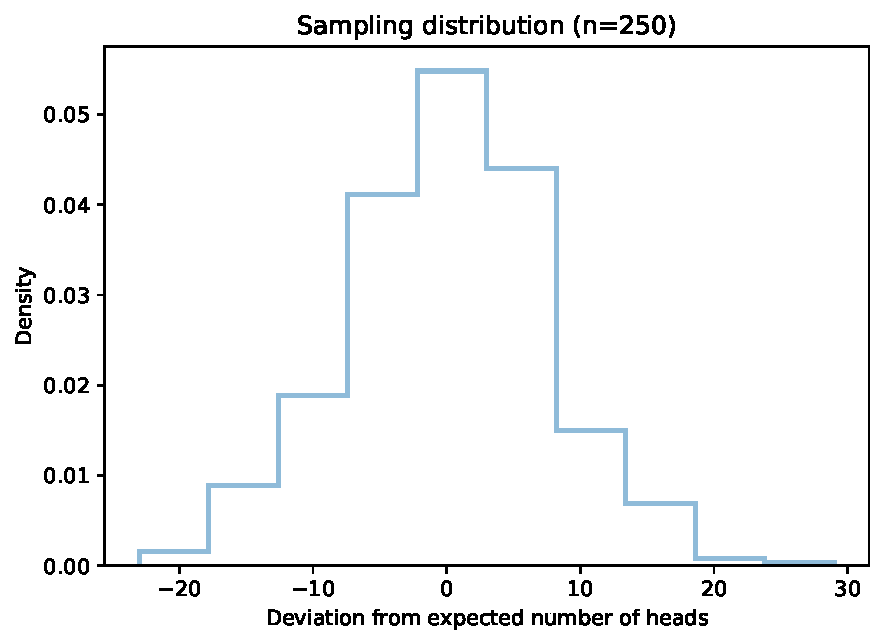
\includegraphics{11_inference_files/11_inference_29_0.pdf}
\caption{png}
\end{figure}

This is the ``sampling distribution'' of deviations. It shows how much
variation we should expect between experiments with this sample size (n
= 250).

\hypertarget{p-values}{%
\section{P-values}\label{p-values}}

Getting get back to the Euro example, Dr.~Bright reported:

``If the coin were unbiased the chance of getting a result as extreme as
that would be less than 7\%''.

The article doesn't say so explicitly, but this is a ``p-value''. To
understand what that means, let's count how many times, in 10000
attempts, the outcome is ``as extreme as'' the observed outcome, 140
heads.

The observed deviation is the difference between the observed and
expected number of heads:

\begin{lstlisting}[language=Python]
observed_diff = heads - expected
observed_diff
\end{lstlisting}

\begin{lstlisting}[]
15.0
\end{lstlisting}

Let's see how many times the simulated \passthrough{\lstinline!diffs!}
exceed the observed deviation:

\begin{lstlisting}[language=Python]
np.mean(diffs >= observed_diff)
\end{lstlisting}

\begin{lstlisting}[]
0.039
\end{lstlisting}

It's around 3\%. But Dr.~Blight said 7\%. Where did that come from?

So far, we only counted the cases where the outcome is \emph{more} heads
than expected. We might also want to count the cases where the outcome
is \emph{fewer} than expected.

Here's the probability of falling below the expected number by 15 or
more.

\begin{lstlisting}[language=Python]
np.mean(diffs <= -observed_diff)
\end{lstlisting}

\begin{lstlisting}[]
0.033
\end{lstlisting}

To get the total probability of a result ``as extreme as that'', we can
use the absolute value of the simulated differences:

\begin{lstlisting}[language=Python]
np.mean(abs(diffs) >= observed_diff)
\end{lstlisting}

\begin{lstlisting}[]
0.072
\end{lstlisting}

So that's consistent with what Dr.~Blight reported.

To show what that looks like graphically, I'll use the following
function, which fills in the histogram between
\passthrough{\lstinline!low!} and \passthrough{\lstinline!high!}.

\begin{lstlisting}[language=Python]
def fill_hist(low, high, patch):
    fill = plt.axvspan(low, high, 
                       clip_path=patch,
                       alpha=0.5, 
                       color='C0')
\end{lstlisting}

The following plot shows the sampling distribution of
\passthrough{\lstinline!diffs!} with two regions shaded. These regions
represent the probability that an unbiased coin yields a deviation from
the expected as extreme as 15.

\begin{lstlisting}[language=Python]
patch = plot_hist(diffs)

# fill the right tail of the hist
low = observed_diff
high = diffs.max()
fill_hist(low, high, patch)

# fill the left tail of the hist
low = diffs.min()
high = -observed_diff
fill_hist(low, high, patch)

plt.title('Sampling distribution (n=250)')
plt.xlabel('Deviation from expected number of heads')
plt.ylabel('Density');
\end{lstlisting}

\begin{figure}
\centering
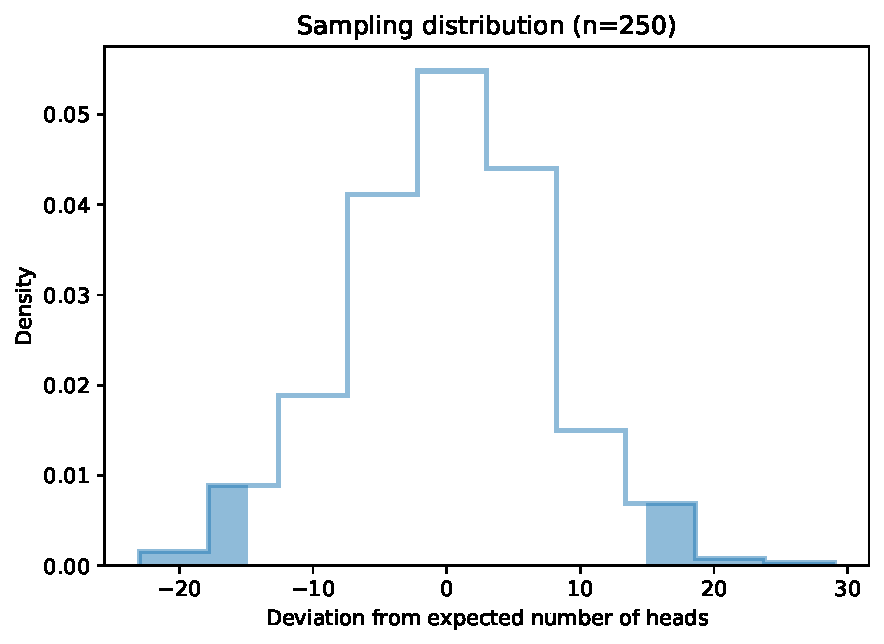
\includegraphics{11_inference_files/11_inference_42_0.pdf}
\caption{png}
\end{figure}

These results show that there is a non-negligible chance of getting a
result as extreme as 140 heads, even if the coin is actually fair.

So even if the results are ``suspicious'' they don't provide compelling
evidence that the coin is biased.

\textbf{Exercise:} There are a few ways to make ``crooked'' dice, that
is, dice that are more likely to land on one side than the others.
Suppose you run a casino and you suspect that a patron is using a die
that comes up 3 more often than it should.

You confiscate the die, roll it 300 times, and 63 times it comes up 3.
Does that support your suspicions?

\begin{itemize}
\item
  To answer this question, use \passthrough{\lstinline!spin!} to
  simulate the experiment, assuming that the die is fair.
\item
  Use a for loop to run \passthrough{\lstinline!spin!} 1000 times and
  store the results in a NumPy array.
\item
  What is the mean of the results from the simulated experiments?
\item
  What is the expected number of 3s if the die is fair?
\item
  Use \passthrough{\lstinline!plot\_hist!} to plot the results. The
  histogram you plot approximates the sampling distribution.
\end{itemize}

\textbf{Exercise:} Continuing the previous exercise, compute the
probability of seeing a deviation from the expected value that is ``as
extreme'' as the observed difference.

For this context, what do you think is the best definition of ``as
extreme''?

Plot the histogram of the random deviations again, and use
\passthrough{\lstinline!fill\_hist!} to fill the region of the histogram
that corresponds to the p-value you computed.

\hypertarget{are-first-babies-more-likely-to-be-late}{%
\section{Are first babies more likely to be
late?}\label{are-first-babies-more-likely-to-be-late}}

The examples so far have been based on coins and dice, which are
relatively simple. In this section we'll look at an example that's based
on real-world data.

Here's the motivation for it: When my wife and I were expecting our
first baby, we heard that first babies are more likely to be late. We
also hear that first babies are more likely to be early. Neither claim
was supported by evidence.

Fortunately, I am a data scientist! Also fortunately, the CDC runs the
National Survey of Family Growth (NSFG), which ``gathers information on
family life, marriage and divorce, pregnancy, infertility, use of
contraception, and men's and women's health.''

I got the data from their web page,
https://www.cdc.gov/nchs/nsfg/index.htm, and wrote some code to get it
into a Pandas Dataframe:

\begin{lstlisting}[language=Python]
import pandas as pd

nsfg = pd.read_hdf('nsfg.hdf5')
nsfg.shape
\end{lstlisting}

\begin{lstlisting}[]
(9358, 11)
\end{lstlisting}

The \passthrough{\lstinline!nsfg!} DataFrame contains 9358 rows, one for
each recorded pregnancy, and 11 columns, one of each of the variables I
selected.

Here are the first few lines.

\begin{lstlisting}[language=Python]
nsfg.head()
\end{lstlisting}

\begin{tabular}{lrrrrrrrrrrr}
\toprule
{} &  caseid &  outcome &  birthwgt\_lb1 &  birthwgt\_oz1 &  prglngth &  nbrnaliv &  agecon &  agepreg &  birthord &  hpagelb &  wgt2013\_2015 \\
\midrule
0 &   60418 &        1 &           5.0 &           4.0 &        40 &       1.0 &    2000 &   2075.0 &       1.0 &     22.0 &   3554.964843 \\
1 &   60418 &        1 &           4.0 &          12.0 &        36 &       1.0 &    2291 &   2358.0 &       2.0 &     25.0 &   3554.964843 \\
2 &   60418 &        1 &           5.0 &           4.0 &        36 &       1.0 &    3241 &   3308.0 &       3.0 &     52.0 &   3554.964843 \\
3 &   60419 &        6 &           NaN &           NaN &        33 &       NaN &    3650 &      NaN &       NaN &      NaN &   2484.535358 \\
4 &   60420 &        1 &           8.0 &          13.0 &        41 &       1.0 &    2191 &   2266.0 &       1.0 &     24.0 &   2903.782914 \\
\bottomrule
\end{tabular}

The variables we need are \passthrough{\lstinline!birthord!}, which
indicates birth order, and \passthrough{\lstinline!prglength!}, which is
pregnancy length in weeks.

I'll make two boolean Series, one for first babies and one for others.

\begin{lstlisting}[language=Python]
firsts = (nsfg.birthord == 1)
others = (nsfg.birthord > 1)

np.sum(firsts), np.sum(others)
\end{lstlisting}

\begin{lstlisting}[]
(3067, 3422)
\end{lstlisting}

We can use the boolean Series to select pregnancy lengths for the two
groups and compute their means:

\begin{lstlisting}[language=Python]
prglngth = nsfg['prglngth']

mean_first = prglngth[firsts].mean() 
mean_other = prglngth[others].mean()

mean_first, mean_other
\end{lstlisting}

\begin{lstlisting}[]
(38.57124225627649, 38.36908240794857)
\end{lstlisting}

Here's the difference in means, in weeks.

\begin{lstlisting}[language=Python]
diff = mean_first - mean_other
diff
\end{lstlisting}

\begin{lstlisting}[]
0.20215984832792344
\end{lstlisting}

Here it is converted to days:

\begin{lstlisting}[language=Python]
diff * 7
\end{lstlisting}

\begin{lstlisting}[]
1.415118938295464
\end{lstlisting}

It looks like first babies are born 1.4 days later than other babies, on
average.

\hypertarget{hypothesis-testing}{%
\section{Hypothesis testing}\label{hypothesis-testing}}

The apparent difference between these groups is based on a random sample
that is much smaller than the actual population. So we can't be sure
that the difference we see in the sample reflects a real difference in
the population. There are two other possibilities we should keep in
mind:

\begin{itemize}
\item
  Systematic errors: The sample might be more likely to include some
  pregancies, and less likely to include others, in a way that causes an
  apparent difference in the sample, even if there is no such difference
  in the population.
\item
  Sampling errors: Even if every pregnancy is equally likely to appear
  in the sample, it is still possible to see a difference in the sample
  that is not in the population, just because of random variation.
\end{itemize}

We can never rule out the possibility of systematic errors, but we
\emph{can} test whether an apparent effect could be explained by random
sampling.

Here's how:

\begin{enumerate}
\def\labelenumi{\arabic{enumi}.}
\item
  First we choose a ``test statistic'' that measures the size of the
  effect; the test statistic in this example is the difference in mean
  pregnancy length.
\item
  Next we define a model of the population under the assumption that
  there is actually no difference between the groups. This assumption is
  called the ``null hypothesis''.
\item
  Then we use the model to compute the distribution of the test
  statistic under the null hypothesis.
\end{enumerate}

We have already done step 1, but to make it easier to repeat, I'll wrap
it in a function.

\begin{lstlisting}[language=Python]
def test_stat(group1, group2):
    """Difference in means.
    
    group1: sequence of values
    group2: sequence of values
    
    returns: float difference in means
    """
    diff = np.mean(group1) - np.mean(group2)
    return diff
\end{lstlisting}

\passthrough{\lstinline!test\_stat!} takes two sequences and computes
the difference in their means.

Here's how we use it to compute the actual difference in the sample.

\begin{lstlisting}[language=Python]
group1 = prglngth[firsts]
group2 = prglngth[others]

actual_diff = test_stat(group1, group2)
actual_diff
\end{lstlisting}

\begin{lstlisting}[]
0.20215984832792344
\end{lstlisting}

Now we have to define the null hypothesis, which is a model of the world
where there is no difference in pregnancy length between first babies
and others.

One way to do that is to put the two groups together and then divide
them up again at random. That way the distribution of pregnancy lengths
is the same for both groups.

I'll use \passthrough{\lstinline!concatenate!} to pool the groups.

\begin{lstlisting}[language=Python]
len(group1), len(group2)
\end{lstlisting}

\begin{lstlisting}[]
(3067, 3422)
\end{lstlisting}

\begin{lstlisting}[language=Python]
pool = np.concatenate([group1, group2])
pool.shape
\end{lstlisting}

\begin{lstlisting}[]
(6489,)
\end{lstlisting}

I'll use \passthrough{\lstinline!shuffle!} to reorder them.

\begin{lstlisting}[language=Python]
np.random.shuffle(pool)
\end{lstlisting}

Then I'll use \passthrough{\lstinline!split!} to make two simulated
groups, the same size as the originals.

\begin{lstlisting}[language=Python]
n = len(group1)
sim_group1, sim_group2 = np.split(pool, [n])
\end{lstlisting}

\begin{lstlisting}[language=Python]
len(sim_group1), len(sim_group2)
\end{lstlisting}

\begin{lstlisting}[]
(3067, 3422)
\end{lstlisting}

Now we can compute the test statistic for the simulated data.

\begin{lstlisting}[language=Python]
test_stat(sim_group1, sim_group2)
\end{lstlisting}

\begin{lstlisting}[]
-0.014237551111094149
\end{lstlisting}

In the simulated data, the distribution of pregnancy lengths is the same
for both groups, so the difference is usually close to 0.

But because it is based on a random shuffle of the groups, we get a
different value each time we run it.

To see what the whole distribution looks like, we can run the simulation
many times and store the results.

\begin{lstlisting}[language=Python]
diffs = np.empty(1000)

for i in range(len(diffs)):
    np.random.shuffle(pool)
    sim_group1, sim_group2 = np.split(pool, [n])
    diffs[i] = test_stat(sim_group1, sim_group2)
\end{lstlisting}

The result is the ``sampling distribution of the test statistic under
the null hypothesis''.

The mean of this distribution should close to zero, because it is based
on the assumption that there is actually no difference between the
groups.

\begin{lstlisting}[language=Python]
np.mean(diffs)
\end{lstlisting}

\begin{lstlisting}[]
0.0021146729470806775
\end{lstlisting}

And here's what the whole distribution looks like.

\begin{lstlisting}[language=Python]
plot_hist(diffs)

plt.xlabel('Difference in mean (weeks)')
plt.title('Distribution of test statistic under null hypothesis');
\end{lstlisting}

\begin{figure}
\centering
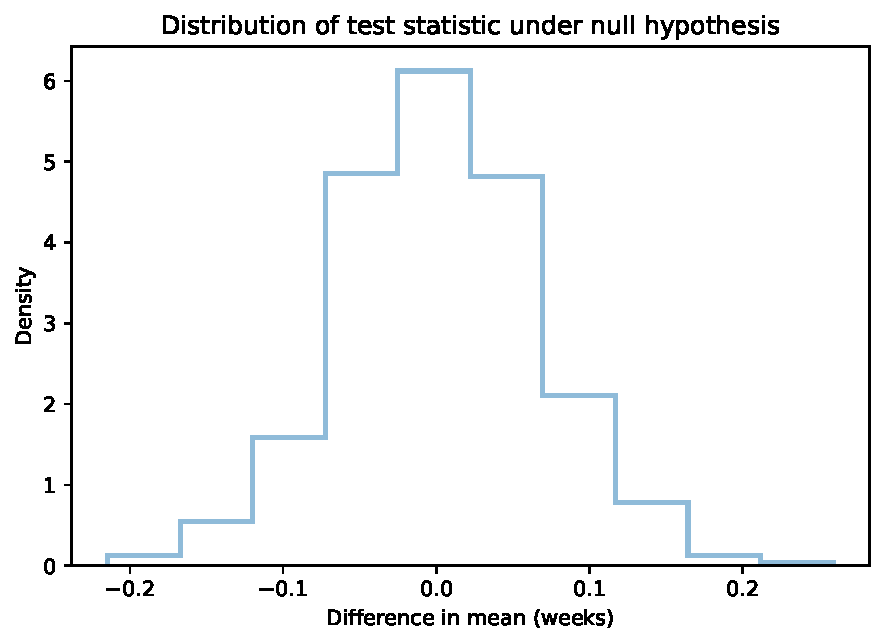
\includegraphics{11_inference_files/11_inference_79_0.pdf}
\caption{png}
\end{figure}

If there were actually no difference between the groups, we would expect
to see a difference as big as 0.15 weeks by chance, at least
occasionally. But a difference as big as 0.2 would be rare.

To quantify that surprise, we can estimate the probability that the test
statistic, under the null hypothesis, exceeds the observed differences
in the means.

The result is a ``p-value''.

\begin{lstlisting}[language=Python]
p_value = np.mean(diffs >= actual_diff)
p_value
\end{lstlisting}

\begin{lstlisting}[]
0.0
\end{lstlisting}

In this example the result is 0, which is to say that in 1000
simulations of the null hypothesis, we never saw a difference as big as
0.2.

\hypertarget{interpreting-p-values}{%
\section{Interpreting p-values}\label{interpreting-p-values}}

To interpret this result, remember that we started with three possible
explanations for the observed difference between the groups:

\begin{enumerate}
\def\labelenumi{\arabic{enumi}.}
\item
  The observed difference might be ``real''; that is, there might be an
  actual difference in pregnancy length between first babies and others.
\item
  There might be no real difference between the groups, and the observed
  difference might be because of a systematic error in the sampling
  process or the data collection process. For example, maybe reported
  pregnancy lengths are less accurate for first time mothers.
\item
  There might be no real difference between the groups, and the observed
  difference might be due to random variation in the sampling process.
\end{enumerate}

By computing a p-value, we have established that it would be rare to see
a difference as big as 0.2 due to sampling alone. So we can conclude
that the third explanation is unlikely.

That makes it more likely that the difference is real, but we still
can't rule out the second possibility.

\textbf{Exercise:} The test statistic we chose is the difference in
means between the two groups.

But suppose we would like to know whether first babies are more
unpredictable than other babies. In that case the test statistic we
choose might be the standard deviation of pregnancy length, which is one
way to quantify unpredictability.

As an exercise:

\begin{enumerate}
\def\labelenumi{\arabic{enumi}.}
\item
  Write a version of \passthrough{\lstinline!test\_stat!} that computes
  the difference in standard deviation between the groups.
\item
  Write a loop that estimates the distribution of this test statistic
  under the null hypothesis.
\item
  Compute a p-value.
\end{enumerate}

\hypertarget{estimation}{%
\section{Estimation}\label{estimation}}

Suppose we want to estimate the average height of men in the U.S.

We can use data from the
\href{https://www.cdc.gov/brfss/index.html}{BRFSS}:

``The Behavioral Risk Factor Surveillance System (BRFSS) is the nation's
premier system of health-related telephone surveys that collect state
data about U.S. residents regarding their health-related risk behaviors,
chronic health conditions, and use of preventive services.''

\begin{lstlisting}[language=Python]
from os.path import basename, exists

def download(url):
    filename = basename(url)
    if not exists(filename):
        from urllib.request import urlretrieve
        local, _ = urlretrieve(url, filename)
        print('Downloaded ' + local)
    
download('https://github.com/AllenDowney/' +
         'ElementsOfDataScience/raw/master/brfss.hdf5')
\end{lstlisting}

\begin{lstlisting}[language=Python]
import pandas as pd

brfss = pd.read_hdf('brfss.hdf5', 'brfss')
brfss.shape
\end{lstlisting}

\begin{lstlisting}[]
(100000, 9)
\end{lstlisting}

We can use \passthrough{\lstinline!SEX!} to select male respondents.

\begin{lstlisting}[language=Python]
male = (brfss.SEX == 1)
np.mean(male)
\end{lstlisting}

\begin{lstlisting}[]
0.48589
\end{lstlisting}

Then we select height data.

\begin{lstlisting}[language=Python]
heights = brfss['HTM4']
data = heights[male]
\end{lstlisting}

We can use \passthrough{\lstinline!isnan!} to check for NaN values:

\begin{lstlisting}[language=Python]
np.mean(np.isnan(data)) * 100
\end{lstlisting}

\begin{lstlisting}[]
4.338430508962934
\end{lstlisting}

About 4\% of the values are missing.

Here are the mean and standard deviation, ignoring missing data.

\begin{lstlisting}[language=Python]
print('Mean male height in cm =', np.nanmean(data))
print('Std male height in cm =', np.nanstd(data))
\end{lstlisting}

\begin{lstlisting}[]
Mean male height in cm = 177.53804780447925
Std male height in cm = 8.350063691943435
\end{lstlisting}

\hypertarget{quantifying-precision}{%
\section{Quantifying precision}\label{quantifying-precision}}

At this point we have an estimate of the average adult male height. We'd
like to know how accurate this estimate is, and how precise. In the
context of estimation, these words have a
\href{https://en.wikipedia.org/wiki/Accuracy_and_precision}{technical
distinction}:

\begin{quote}
Given a set of data points from repeated measurements of the same
quantity, the set can be said to be precise if the values are close to
each other, while the set can be said to be accurate if their average is
close to the true value of the quantity being measured.
\end{quote}

Usually accuracy is what we really care about, but it's hard to measure
accuracy unless you know the true value. And if you know the true value,
you don't have to estimate it.

Quantifying precision is not as useful, but it is much easier. Here's
one way to do it:

\begin{enumerate}
\def\labelenumi{\arabic{enumi}.}
\item
  Use the data you have to make a model of the population.
\item
  Use the model to simulate the data collection process.
\item
  Use the simulated data to compute an estimate.
\end{enumerate}

By repeating these steps, we can quantify the variability of the
estimate due to random sampling.

To model the population, I'll use \textbf{resampling}; that is, I will
treat the observed measurements as if they were taken from the entire
population, and I will draw random samples from them.

We can use \passthrough{\lstinline!np.random.choice!} to resample the
data:

\begin{lstlisting}[language=Python]
size = len(data)
sim_data = np.random.choice(data, size, replace=True)
sim_data.shape
\end{lstlisting}

\begin{lstlisting}[]
(48589,)
\end{lstlisting}

With \passthrough{\lstinline!replace=True!}, we sample with replacement,
which means that some measurements might be chosen more than once, and
some might not be chosen at all.

(If we sample \emph{without} replacement, the resampled data is always
identical to the original, so that's no good.)

Now we can use \passthrough{\lstinline!nanmean!} to compute the mean of
the simulated data, ignoring missing values.

\begin{lstlisting}[language=Python]
np.nanmean(sim_data)
\end{lstlisting}

\begin{lstlisting}[]
177.52799586999075
\end{lstlisting}

If we repeat this process 1000 times, we can see how much the results
vary.

\begin{lstlisting}[language=Python]
outcomes = np.empty(1000)
size = len(data)

for i in range(len(outcomes)):
    sim_data = np.random.choice(data, size, replace=True)
    outcomes[i] = np.nanmean(sim_data)
\end{lstlisting}

The result is the ``sampling distribution'', which shows how much the
results of the experiment would vary if we ran it many times. Here's
what it looks like:

\begin{lstlisting}[language=Python]
plot_hist(outcomes)
plt.title('Sampling distribution of the mean')
plt.xlabel('Mean adult male height, U.S.');
\end{lstlisting}

\begin{figure}
\centering
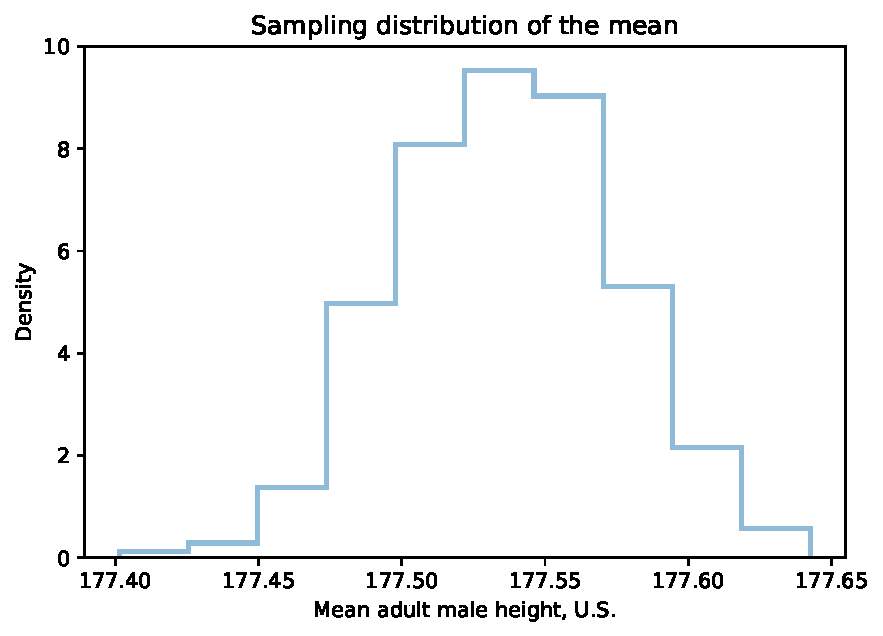
\includegraphics{11_inference_files/11_inference_105_0.pdf}
\caption{png}
\end{figure}

The width of this distribution shows how much the results vary from one
experiment to the next.

We can quantify this variability by computing the standard deviation of
the sampling distribution, which is called ``standard error''.

\begin{lstlisting}[language=Python]
std_err = np.std(outcomes)
std_err
\end{lstlisting}

\begin{lstlisting}[]
0.038376132495234826
\end{lstlisting}

We can also summarize the sampling distribution with a ``confidence
interval'', which is a range that contains a specified fraction, like
90\%, of the values in \passthrough{\lstinline!sampling\_dist\_mean!}.

The central 90\% confidence interval is between the 5th and 95th
percentiles of the sampling distribution.

\begin{lstlisting}[language=Python]
ci_90 = np.percentile(outcomes, [5, 95])
ci_90
\end{lstlisting}

\begin{lstlisting}[]
array([177.47655879, 177.60152771])
\end{lstlisting}

The following function plots a histogram and shades the 90\% confidence
interval.

\begin{lstlisting}[language=Python]
def plot_sampling_dist(outcomes):
    """Plot sampling distribution.
    
    outcomes: sequence of values
    """
    patch = plot_hist(outcomes)
    low, high = np.percentile(outcomes, [5, 95])
    fill_hist(low, high, patch)
    print('Mean = ', np.mean(outcomes))
    print('Std error = ', np.std(outcomes))
    print('90% CI = ', (low, high))
\end{lstlisting}

Here's what it looks like for the sampling distribution of mean adult
height:

\begin{lstlisting}[language=Python]
plot_sampling_dist(outcomes)
plt.xlabel('Mean adult male height, U.S. (%)');
\end{lstlisting}

\begin{lstlisting}[]
Mean =  177.5401473153372
Std error =  0.038376132495234826
90% CI =  (177.47655879241216, 177.60152770795776)
\end{lstlisting}

\begin{figure}
\centering
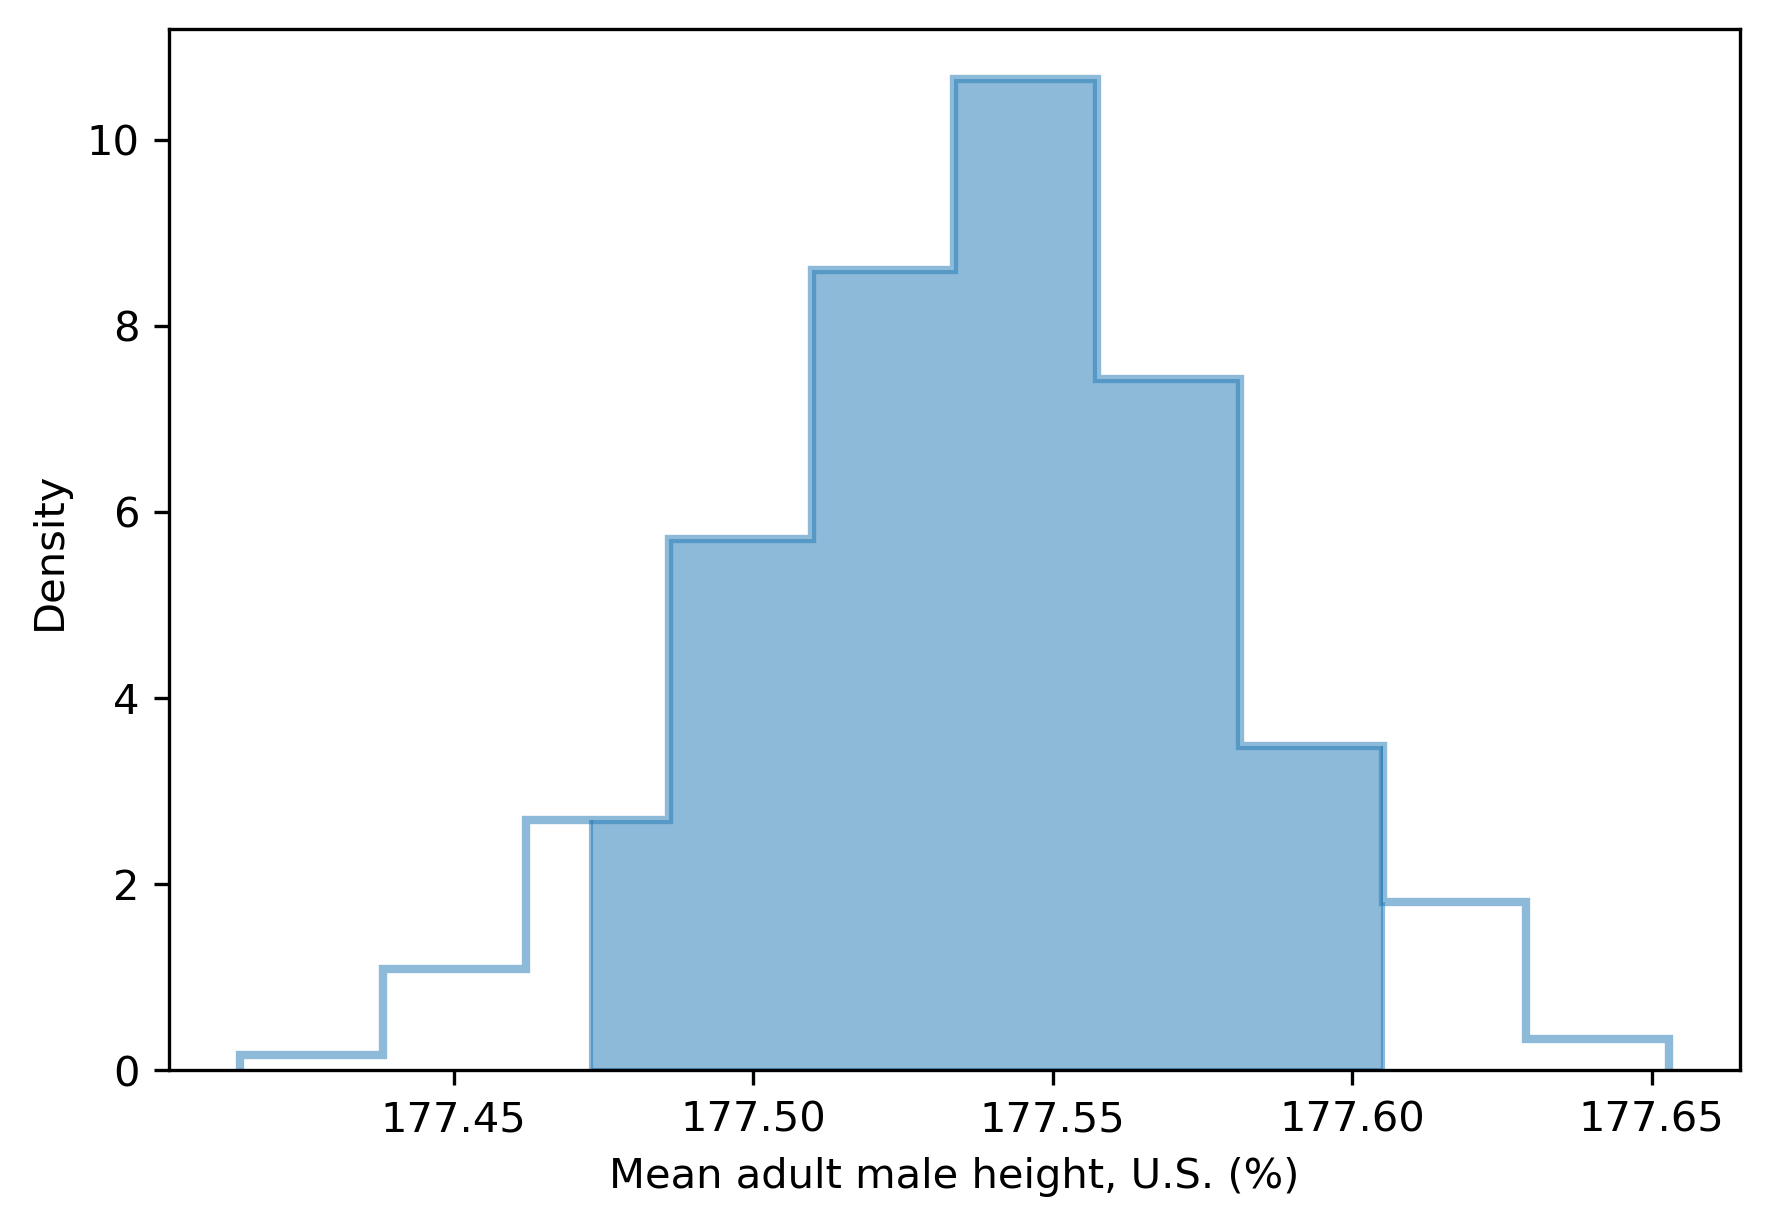
\includegraphics{11_inference_files/11_inference_113_1.png}
\caption{png}
\end{figure}

For an experiment like this, we can compute the standard error
analytically.

\begin{lstlisting}[language=Python]
size = len(data)
analytic_std_err = np.std(data) / np.sqrt(size)
\end{lstlisting}

The result is close to what we observed computationally.

\begin{lstlisting}[language=Python]
analytic_std_err, std_err
\end{lstlisting}

\begin{lstlisting}[]
(0.03788094526418763, 0.038376132495234826)
\end{lstlisting}

This result indicates that our estimate of the mean is \emph{precise};
that is, if we ran this experiment many times, the results would fall in
a narrow range.

But this range reflects only variability due to random sampling. If
there are systematic errors in the sampling process, or in the
measurement process, the result would not be \emph{accurate}.

Computing a standard error or confidence interval can be useful, but it
only quantifies variability due to random sampling, not other sources of
error.

\textbf{Exercise:} One nice thing about using resampling is that it is
easy to compute the sampling distribution for other statistics.

For example, suppose we want to estimate the coefficient of variation
(standard deviation as a fraction of the mean) for adult male height.
Here's how we can compute it.

\begin{lstlisting}[language=Python]
cv = np.nanstd(data) / np.nanmean(data)
cv
\end{lstlisting}

\begin{lstlisting}[]
0.04703253074596872
\end{lstlisting}

So the standard deviation is about 5\% of the mean.

Write a loop that uses resampling to estimate the sampling distribution
of \passthrough{\lstinline!cv!}; store the results in an array named
\passthrough{\lstinline!outcomes!}.

Then use \passthrough{\lstinline!plot\_sampling\_dist!} to plot the
sampling distribution of the coefficient of variation.

What is the standard error of the estimated coefficient of variation?

\hypertarget{summary}{%
\section{Summary}\label{summary}}

This chapter presents computational methods for computing p-values,
standard errors, and confidence intervals. The two processes are
similar, but they answer different questions.

The following diagram outlines the hypothesis testing process:

Again, the key steps are

\begin{enumerate}
\def\labelenumi{\arabic{enumi}.}
\item
  Choose a test statistic that quantifies the observed effect.
\item
  Define a model of the null hypothesis and use it to generate simulated
  data.
\item
  Compute the distribution of the test statistic under the null
  hypothesis.
\item
  Compute a p-value, which is probability, under the null hypothesis, of
  seeing an effect as extreme as what you saw.
\end{enumerate}

The following figure shows the similar process for computing standard
errors and confidence intervals.

The essential steps are:

\begin{enumerate}
\def\labelenumi{\arabic{enumi}.}
\item
  Choose a sample statistic that quantifies the thing you want to
  estimate.
\item
  Use the data to make a model of the population, assuming that the
  estimate is accurate.
\item
  Use the model to simulate the sampling process and generate simulated
  data.
\item
  Compute the sampling distribution of the estimate.
\item
  Use the sampling distribution to compute the standard error,
  confidence interval, or both.
\end{enumerate}

Finally, remember that both processes only account for variability due
to random sampling. They don't tell us anything about systematic errors
in the sampling process, measurement error, or other sources of error.

